%!TEX root = book.tex

\chapter{Answers to the Problem Sets}

\newslide
\problemset

\newslide

\begin{problem}
(a) The redshift is $z = 1.82 \times 10^{-9}$. (b) Rounding errors from a
typical single-precision floating-point number are two orders
of magnitude larger than this.
\end{problem}

\newslide

\begin{problem}
\begin{enumerate}
\item[(a)] The photon distribution function is the phase-space density
  of photons. Therefore, the total space-density of photons $N$ can be
  obtained by integrating the photon distribution function over all
  momenta. That is,
\begin{align}
N &= \int_0^\infty\!\!\!dp^3\:f(\vec r,\vec p)\\
  &= \int_0^\infty\!\!\!dp \int_{4\pi}\!\!\! d\Omega\: p^2 f(\vec r,\vec p).
\end{align}
We then substitute $p = h\nu/c$ and $f = c^2I_\nu/h^4\nu^3$ to obtain
\begin{align}
N = \frac{1}{h c} 
\int_0^\infty\!\!\!d\nu\int_{4\pi}\!\!\!d\Omega\:\frac{I_\nu}{\nu}.
\end{align}
Since $\nu$ is independent of direction, this is
\begin{align}
N = \frac{4\pi}{h c} \int_0^\infty\!\!\!d\nu\:\frac{J_\nu}{\nu}.
\end{align}
\item[(b)] Similarly, the total energy density $E$ can be obtained by
  integrating the product of the photon distribution function and the
  energy per photon $h\nu$. That is,
\begin{align}
E &= \int_0^\infty\!\!\!dp^3\:h\nu f(\vec r,\vec p).
\end{align}
Using the same substitutions as above, we obtain
\begin{align}
E = \frac{4\pi J}{c}.
\end{align}

\end{enumerate}
\end{problem}

\newslide

\begin{problem}

\begin{figure}[bp]
\centering
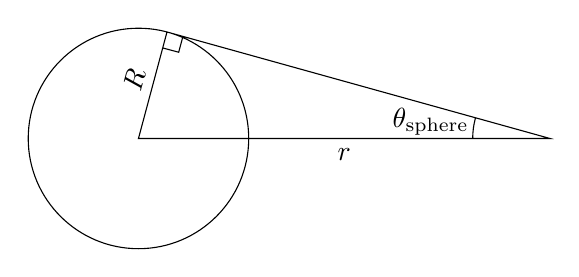
\begin{tikzpicture}[scale=0.7]
\draw
  (0,0) circle (2.0)
  (7.464,0) -- node [pos=0.5,below] {$r$} (0,0) -- node [pos=0.5,above,sloped] {$R$} (75:2.0) -- cycle
  (7.464,0) ++ (-1.4,0) arc (180:165:1.4)
  (75:2.0) ++(-105:0.3) -- ++(-15:0.3) -- ++(75:0.3);
  \node at (5.3,0.3) {$\theta_\mathrm{sphere}$};
\end{tikzpicture}
\caption{The geometry of the proof of the inverse square law.}
\label{fig-inverse-square-law}
\end{figure}

Consider Figure \ref{fig-inverse-square-law}, which shows a right
triangle formed by the line from the center of the sphere to a point $r$
from the center, the tangent to the sphere passing through this point,
and the radius that is normal to the tangent. From the conservation of
intensity, the intensity on rays that intersect the sphere is $I$ and on
rays that do not intersect the sphere is 0. Thus, the radial flux is
given by
\begin{align}
F(r) = I \int_{\Omega_\mathrm{sphere}}\!\!\!\!\!\!d\Omega
\cos\theta,
\end{align}
where $\Omega_\mathrm{sphere}$ is the solid angle of the
sphere and $\theta$ is the angle between the ray and the
radius. Changing variables, this becomes
\begin{align}
F(r) &= I
\int_0^{2\pi}\!\!\!d\phi\:
\int_0^{\theta_\mathrm{sphere}}\!\!\!d\theta \sin\theta
\cos\theta\\
&=
2\pi I \left[\frac{\sin^2\theta}{2}\right]_0^{\theta_\mathrm{sphere}}\\
&=
\pi I \sin^2\theta_\mathrm{sphere}.
\end{align}
However, we have $\sin\theta_\mathrm{sphere} = R / r$, and so
\begin{align}
F(r) = \pi R^2 I / r^2,
\end{align}
and we recover the inverse square law.

The flux at the surface $r = R$ is $F(R) = \pi I$, which is
identical to the result for the flux at a plane-parallel
surface that emits isotropically outwards.

\end{problem}

\newslide

\begin{problem}
The geometry is plane-parallel. Therefore, we have
\begin{align}
F_\nu &= 2\pi\int_{-1}^{+1}\!\!\!d\mu\:\mu I_\nu(\mu),\\
      &= 2\pi I_\nu(1)\int_{0}^{+1}\!\!\!d\mu\:\mu,\\
      &= \pi I_\nu(1).
\end{align}
\end{problem}

%\begin{problem}
%We define
%\begin{align}
%I_\nu &\equiv I_0 + f(\mu),\\
%\intertext{in which}
%f(\mu) &= 
%\begin{cases}
%+g(+\mu)&\mbox{for $\mu \ge 0$, and}\\
%-g(-\mu)&\mbox{for $\mu <   0$.}
%\end{cases}
%\end{align}
%Thus, $f(\mu)$ and also $\mu^2f(\mu)$ are odd functions. We then have
%\begin{align}
%J_\nu 
%&= \frac{1}{2}\int_{-1}^{+1}\!\!\!d\mu\:I_\nu(\mu)\\
%&= \frac{1}{2}\int_{-1}^{+1}\!\!\!d\mu\:I_0
%+ \frac{1}{2}\int_{-1}^{+1}\!\!\!d\mu\:f(\mu)\\
%&= I_0
%\intertext{and}
%K_\nu 
%&= \frac{1}{2}\int_{-1}^{+1}\!\!\!d\mu\:I_\nu(\mu)\mu^2\\
%&= \frac{1}{2}\int_{-1}^{+1}\!\!\!d\mu\:I_0\mu^2
%+ \frac{1}{2}\int_{-1}^{+1}\!\!\!d\mu\:f(\mu)\mu^2\\
%&= \frac{I_0}{3}.
%\end{align}
%In these, we have used the fact that the integral of an odd function over a symmetric 
%interval is zero.
%Therefore, $f = 1/3$.
%\end{problem}

%\begin{problem}
%\begin{enumerate}
%\item[(a)]
%We have
%\begin{align}
%K_\nu \equiv
%\int_{-1}^{+1}\!\!\!d\mu\:I_\nu\mu^2.
%\end{align}
%In the range of integration $\mu$ satisfies $0 \le \mu^2\le 1$ and
%$I_\nu$ is positive. Therefore, in the range of integration, we have 
%\begin{align}
%0 \le I_\nu\mu^2 \le I_\nu.
%\end{align}
%and so
%\begin{align}
%\int_{-1}^{+1}\!\!\!d\mu\:0
%&\le
%\int_{-1}^{+1}\!\!\!d\mu\:I_\nu\mu^2\\
%0 
%&\le
%K\nu\\
%\intertext{and}
%\int_{-1}^{+1}\!\!\!d\mu\:I_\nu\mu^2
%&\le
%\int_{-1}^{+1}\!\!\!d\mu\:I_\nu\\
%K_\nu
%&\le
%J_\nu.
%\end{align}
%Thus,
%\begin{align}
%0 \le K_\nu \le J_\nu.
%\end{align}
%Substituting $K_\nu \equiv f J_\nu$, we find
%\begin{align}
%0 \le f J_\nu \le J_\nu.
%\end{align}
%Thus, provided $J_\nu > 0$, we have
%\begin{align}
%0 \le f \le 1.
%\end{align}
%
%\item[(b)]
%$I_\nu(\mu) \propto \delta(\mu)$ has $f = 0$ and $I_\nu(\mu)
%  \propto\delta(\mu - 1)$ has $f = 1$. (Here, $\delta$ is the Dirac
%  $\delta$ function.)
%
%\end{enumerate}
%\end{problem}

%\begin{problem}
%Since the radiation is isotropic, the total radiation pressure is given
%by
%\begin{align}
%p = \frac{4\pi J}{3}.
%\end{align}
%Using the same reasoning that lead to the interpretation of the
%radiation pressure as the flux of momentum and again since the radiation
%is isotropic, we find that the total flux of momentum that impinges on
%the wall is
%\begin{align}
%\frac{1}{c}
%\int_0^\infty\!\!\!d\nu
%\int_{2\pi}\!\!\!d\Omega
%\:I_\nu\cos^2\theta
%= 
%\frac{2\pi J}{3c} = \frac{p}{2}.
%\end{align}
%in which $\theta$ is the angle to the normal to the wall and we
%integrate over only the inward $2\pi$ steradians because we wish to
%consider only the impinging photons.
%\begin{enumerate}
%\item[(a)] 
%If the photons are reflected, each photon undergoes a change in its
%momentum perpendicular to the wall of $2(h\nu/c)\cos\theta$. This is
%twice its contribution to the flux of momentum that impinges on the
%wall. Therefore, the force per unit area of the wall is
%\begin{align}
%\frac{4\pi J}{3c} = p.
%\end{align}
%\item[(b)]
%If the walls are transparent, no photon undergoes any change in its
%momentum. Therefore, the force per unit area of the wall is zero.
%\item[(c)]
%If the walls are perfect partial mirrors with reflectivity $R$, on
%average each photon undergoes a change in its momentum perpendicular to
%the wall of $2R(h\nu/c)\cos\theta$. This is twice its contribution to
%the flux of momentum that impinges on the wall. This is $2R$ times its
%contribution to the flux of momentum that impinges on the wall.
%Therefore, the force per unit area of the wall is
%\begin{align}
%\frac{4R\pi J}{3c} = R p.
%\end{align}
%\item[(d)]
%If the walls are perfect absorbers, each photon undergoes a change in
%its component of momentum perpendicular to the wall of
%$(h\nu/c)\cos\theta$. This is exactly its contribution to the flux of
%momentum that impinges on the wall. Therefore, the force per unit area
%of the wall is
%\begin{align}
%\frac{2\pi J}{3c} = \frac{p}{2}.
%\end{align}
%\item[(e)] 
%The analogs of these cases for a gas of massive particles are (a) the
%particles are reflected elastically; (b) the particles pass through the
%walls; (c) a fraction $R$ are reflected elastically and a fraction $1-R$
%pass through the walls; and (d) the particles are absorbed
%inelastically.
%\end{enumerate}
%\end{problem}

%\begin{problem}
%The total luminosity $L$ and total flux $F$ at the surface of the Sun
%are related by $L=4\pi R^2F$ and the effective temperature
%$T_\mathrm{eff}$ is defined by $F\equiv\sigma T_\mathrm{eff}^4$. Thus,
%$T_\mathrm{eff} = (L/4\pi R^2\sigma)^{1/4}$, which for the Sun is 5770
%K.
%\end{problem}
%
%\begin{problem}
%The total luminosity of Arcturus is $L = 4\pi R^2\sigma
%T_\mathrm{eff}^4$ and the total flux $F$ at the Earth is $F = L/4\pi
%d^2$, where $d$ is the distance to Arcturus. Thus, the effective
%temperature is given by $T_\mathrm{eff} = (F d^2 / \sigma R^2)^{1/4} =
%(F/ \sigma \alpha^2 )^{1/4}$, where $\alpha$ is the angular radius of
%Arcturus. Thus, the single piece of information we need is the angular
%radius. \citet{quirrenbach-1996} determine an angular diameter of
%$21.0$ milliarcsec using an optical interferometer. This leads to an
%effective temperature of 4290 K. See \citet{griffin-1999} for a
%discussion of the uncertainties.
%\end{problem}

\newslide

\begin{problem}
We are allowed to assume that $\theta^1$ Ori emits isotropically with $I_\nu = B_\nu$. We define the solid angle of $\theta^1$ Ori to be $\Omega$.
Since $\Omega \ll 1$, we have $F_\nu \approx B_\nu\Omega$. In terms of the angular diameter $\alpha$, we have $\Omega = (\pi/4) \alpha^2$ and $\alpha \approx (4F_\nu/\pi B_\nu)^{1/2}$. We now need $F_\nu$ and $B_\nu$. 

\cite{Bessell-2012} define $\mbox{mag}_x = AB - ZP_x$ (their equation 1) and give $ZP_V = -0.023$ (their table 3). Thus, $\theta^1$ Ori with $V = 5.1$ has $AB = 5.077$ and $F_\nu = 3631 \times 10^{-0.4 \times 5.1}~\mathrm{Jy} = 33.1~\mathrm{Jy} = 3.31\times 10^{-22}~\mathrm{erg\,s^{-1}\,cm^{-2}\,Hz^{-1}}$.

In the Rayleigh-Jeans tail, $B_\nu = 2kT\nu^2/c^2$. \cite{Bessell-2012} give the effective wavelength of $V$ as 5455~{\AA} which corresponds to $5.5 \times 10^{14}~\mathrm{Hz}$. At 45,500~K, $B_\nu = 4.22 \times 10^{-3}~\mathrm{erg\,s^{-1}\,cm^{-2}\,Hz^{-1}}$.

Thus, $\alpha = 3.2\times 10^{-10}~\mathrm{rad} = 0.066~\mathrm{mas}$.

%The zero-point flux in $V$ is 3631 Jy. Thus, the flux $F_V$ of $\theta^1$ Ori is $3631\ \mbox{Jy} \times 10^{-0.4 \times 5.1} = 33\ \mbox{Jy} = $. 

\end{problem}

\newslide

\problemset

\newslide

\begin{problem}
\begin{enumerate}
\item[(a)]
The probability density function $p(x)$ is defined such that  the probability that an event in the interval $(x,x+dx)$ is $p(x)dx$. Thus, in terms of the probability $P(>\!x$) that an event occurs after $x$, we have
\begin{align}
p(x)dx = P(>\!x) - P(>\!(x+dx)),
\end{align}
and so
\begin{align}
p(x) &= - \left[\frac{P(>\!(x+dx)) - P(>\!x)}{dx}\right],\\
&= - \frac{dP(>\!x)}{dx}.
\end{align}
\item[(b)]
We have
\begin{align}
\frac{dI_\nu}{d\tau}&= S_\nu - I_\nu,\\
\intertext{but in the absence of emission $S_\nu = 0$, so}
\frac{dI_\nu}{d\tau}&= - I_\nu,\\
\intertext{which can be integrated to give}
\left.\log I_\nu\right|_0^\tau &= -\left.\tau\right|_0^\tau\\
\intertext{or}
I_\nu(\tau) &= e^{-\tau}I_\nu(0).
\end{align}
The number of photons in the beam is proportional to the intensity which falls as $e^{-\tau}$. Thus, the probability $P(>\!\tau)$ that a photon travels an optical depth of at least $\tau$ before being extinguished is also proportional to $e^{-\tau}$. That is,
\begin{align}
P(\>\!\tau) \propto e^{-\tau}.
\end{align}
Since all photons travel at least an optical depth of 0, we have 
\begin{align}
P(>\!0) = 1,
\end{align}
and so the constant of proportionality is 1 and we have
\begin{align}
P(>\!\tau) = e^{-\tau}.
\end{align}
From the result of (a), we the probability density function is 
\begin{align}
p(\tau) = -\frac{dP(>\!\tau)}{d\tau} = -\frac{e^{-\tau}}{d\tau} = e^{-\tau}.
\end{align}
This is an exponential distribution.
\item[(c)]
The mean number of optical depth for extinction $\bar\tau$ is then given by
\begin{align}
\bar\tau &=  \int_{0}^\infty\!\!\!d\tau\:p(\tau)\tau\\
&=\int_{0}^\infty\!\!\!d\tau\:e^{-\tau}\tau\\
&=\left[-e^{-\tau}\tau + \int\!\!\!d\tau\:e^{-\tau}\right]_0^\infty\\
&=\left[-e^{-\tau}\tau -e^{-\tau}\right]_0^\infty\\
&=1.
\end{align}
Thus, the mean optical depth travelled by each photon $\bar\tau$ is 1.
\end{enumerate}
\end{problem}

%\begin{problem}
%By applying $\frac{1}{4\pi}\int_{4\pi}\!d\Omega=\frac{1}{2}\int_{-1}^{+1}\!\!\!d\mu$ to the radiation transfer equation in plane-parallel symmetry and using the isotropy of $S_\nu$, we obtain
%\begin{align}
%\frac{1}{2}\int_{-1}^{+1}\!\!\!d\mu\:\mu\frac{dI\nu}{d\tau} &=
%\frac{1}{2}\int_{-1}^{+1}\!\!\!d\mu\:I_\nu -
%\frac{1}{2}\int_{-1}^{+1}\!\!\!d\mu\:S_\nu\\
%\frac{d}{d\tau}\frac{1}{2}\int_{-1}^{+1}\!\!\!d\mu\:\mu I_\nu &=
%\frac{1}{2}\int_{-1}^{+1}\!\!\!d\mu\:I_\nu -
%S_\nu\frac{1}{2}\int_{-1}^{+1}\!\!\!d\mu\\
%\frac{dH}{d\tau} &=
%J_\nu -
%S_\nu.
%\end{align}
%Similarly, by applying $\frac{1}{4\pi}\int_{4\pi}\!d\Omega\:\mu=\frac{1}{2}\int_{-1}^{+1}\!\!\!d\mu\:\mu$, we obtain
%\begin{align}
%\frac{1}{2}\int_{-1}^{+1}\!\!\!d\mu\:\mu^2\frac{dI\nu}{d\tau} &=
%\frac{1}{2}\int_{-1}^{+1}\!\!\!d\mu\:\mu I_\nu -
%\frac{1}{2}\int_{-1}^{+1}\!\!\!d\mu\:\mu S_\nu\\
%\frac{d}{d\tau}\frac{1}{2}\int_{-1}^{+1}\!\!\!d\mu\:\mu^2 I_\nu &=
%\frac{1}{2}\int_{-1}^{+1}\!\!\!d\mu\:\mu I_\nu -
%S_\nu\frac{1}{2}\int_{-1}^{+1}\!\!\!d\mu\:\mu\\
%\frac{dK}{d\tau} &=
%H_\nu.
%\end{align}
%\end{problem}
%
%\begin{problem}
%We can define the moment $M_m(I_\nu)$ in terms of the upwards and downwards components $M_m^+(I_\nu)$ and $M_m^-(I_\nu)$ as
%\begin{align}
%M_m(I_\nu) 
%&\equiv M_m^+(I_\nu) + M_m^-(I_\nu)\\
%&\equiv \frac{1}{2}\int_0^{+1}\!\!\!d\mu\:\mu^mI_\nu  + \frac{1}{2}\int_{-1}^{0}\!\!\!d\mu\:\mu^mI_\nu.
%\end{align}
%Substituting the formal solution for $I_\nu$ and making the substitutions $w = \mu$ in the first integral and $w = -\mu$ in the second integral, we obtain
%\begin{align}
%M_m^+(I_\nu) 
%&= \frac{1}{2}\int_\tau^\infty\!\!\!dt S_\nu(t) \int_1^\infty\!\!\!\frac{dw}{w^{m+1}}\:e^{w(\tau-t)}\\
%&= \frac{1}{2}\int_\tau^\infty\!\!\!dt S_\nu(t) E_{m+1}(|t-\tau|)\\
%\intertext{and}
%M_m^-(I_\nu) 
%&= (-1)^{m+1}\frac{1}{2}\int_0^\tau\!\!\!dt S_\nu(t) \int_1^\infty\!\!\!\frac{dw}{w^{m+1}}\:e^{w(t-\tau)}\\
%&= (-1)^{m+1}\frac{1}{2}\int_0^\tau\!\!\!dt S_\nu(t) E_{m+1}(|t-\tau|).
%\end{align}
%Thus,
%\begin{align}
%M_m(I_\nu) 
%&=
%\frac{1}{2}\int_\tau^\infty\!\!\!dt S_\nu(t) E_{m+1}(|t-\tau|)
%+ 
%(-1)^{m+1}\frac{1}{2}\int_0^\tau\!\!\!dt S_\nu(t) E_{m+1}(|t-\tau|).
%\end{align}
%
%\end{problem}
%

\newslide

\begin{problem}
The radiation transfer equation in plane-parallel geometry is
\begin{align}
\mu \frac{d I_\nu}{dz} = j_\nu - \chi I_\nu.
\end{align}
Integrating over frequency and solid angle, gives
\begin{align}
\frac{1}{2}\int_0^\infty\!\!\!d\nu\int_{-1}^{+1}\!\!\!d\mu\:\mu\frac{d I_\nu}{dz} 
&=
\frac{1}{2}\int_0^\infty\!\!\!d\nu\int_{-1}^{+1}\!\!\!d\mu\:j_\nu -
\frac{1}{2}\int_0^\infty\!\!\!d\nu\int_{-1}^{+1}\!\!\!d\mu\:\chi I_\nu
\end{align}
If we assume that $j_\nu$ and $\chi$ are isotropic, then
\begin{align}
\frac{d}{dz} \frac{1}{2}\int_0^\infty\!\!\!d\nu\int_{-1}^{+1}\!\!\!d\mu\:\mu I_\nu
&=
\frac{1}{2}\int_0^\infty\!\!\!d\nu\:j_\nu\int_{-1}^{+1}\!\!\!d\mu -
\frac{1}{2}\int_0^\infty\!\!\!d\nu\:\chi\int_{-1}^{+1}\!\!\!d\mu I_\nu\\
\frac{d}{dz}\int_0^\infty\!\!\!d\nu\:H_\nu
&=
\int_0^\infty\!\!\!d\nu\:j_\nu -
\int_0^\infty\!\!\!d\nu\:\chi J_\nu\\
\frac{dH}{dz}
&=
\int_0^\infty\!\!\!d\nu\:j_\nu -
\int_0^\infty\!\!\!d\nu\:\chi J_\nu\\
\frac{1}{4\pi}\frac{dF}{dz}
&=
\int_0^\infty\!\!\!d\nu\:j_\nu -
\int_0^\infty\!\!\!d\nu\:\chi J_\nu
\end{align}
Thus, $dF/dz = 0$ implies and is implied by $\int_0^\infty\!\!\!d\nu\:j_\nu =
\int_0^\infty\!\!\!d\nu\:\chi J_\nu$.
\end{problem}

\newslide

\begin{problem}
The formal solution to the radiation transfer equation for $\mu > 0$ at the surface of a plane-parallel atmosphere is
\begin{align}
I_\nu(0,\mu) 
&= \int_0^\infty\!\!\!\frac{d\tau}{\mu}\:e^{-\tau/\mu}S_\nu(\tau).
\end{align}
Substituting $S_\nu = a + b\tau$ and $x \equiv \tau/\mu$, gives
\begin{align}
I_\nu(0,\mu) 
&= \int_0^\infty\!\!\!\frac{d\tau}{\mu}\:e^{-\tau/\mu}(a + b\tau)\\
&= \int_0^\infty\!\!\!dx\:e^{-x}(a + b\mu x)\\
&= \left[-ae^{-x} - b\mu xe^{-x} +b\mu \int\!\!\!dx e^{-x}\right]_0^\infty\\
&= \left[-ae^{-x} - b\mu xe^{-x} -b\mu e^{-x}\right]_0^\infty\\
&= a + b\mu\\
&= S_\nu(\tau = \mu).
\end{align}
From the definition of $F$, the upper boundary condition that $I(0,\mu) = 0$ for $\mu < 0$, and the Eddington-Barbier relation $I(0,\mu) = S_\nu(\tau=\mu)$ for $\mu > 0$, we have
\begin{align}
F_\nu(0) &= 2\pi\int_0^{+1}\!\!\!d\mu\:\mu S(\tau=\mu)\\
&= 2\pi\int_0^{+1}\!\!\!d\mu\:\mu(a + b\mu)\\
&=2\pi\left[\frac{a\mu^2}{2} + \frac{b\mu^3}{3}\right]_0^{+1}\\
&=2\pi\left[\frac{a}{2}+\frac{b}{3}\right]\\
&=\pi\left[a + \frac{2}{3}b\right]\\
&=\pi S_\nu(\tau=2/3).
\end{align}
\end{problem}

\newslide

\begin{problem}
\begin{enumerate}
%\item[(a)]
%From the formal solution for $I_\lambda$ at the surface,
%\begin{align}
%I_\lambda(0,\mu)
%=
%\int_0^\infty\!\!\!\frac{d\tau}{\mu}\:
%e^{-\tau/\mu}
%\sum a_n \tau^n.
%\end{align}
%Making the substitution $x \equiv \tau / \mu$ and
%interchanging the integral and the sum, gives
%\begin{align}
%I_\lambda(0,\mu)
%&=
%\sum 
%a_n\mu^n
%\int_0^\infty\!\!\!{dx}\: e^{-x}
%x^n\\
%&=
%\sum 
%a_n \mu^n
%\Gamma(n + 1)\\
%&=
%\sum 
%a_n \mu^n n!.
%\end{align}

\item[(a)]
From the generalization of the Eddington-Barbier relations, we have $S_\lambda(\tau) =
I_\lambda(0,0)[a_0 + a_1\tau + a_2\tau^2]$ for $\tau \le 1$. 
In LTE and in the absence of scattering, we further have $S_\lambda = B_\lambda$.

Thus, the optical depth
$\tau(T)$ to a given temperature $T$ and the temperature $T(\tau)$ at a given optical depth
are given implicitly by
\begin{align}
B_\lambda(T) = I_\lambda(0,0)[a_0 + a_1\tau + a_2\tau^2].
\end{align}
\item[(b)]
From the definition of optical depth, we have \begin{align}
\chi = - \frac{d\tau}{dz} = - \frac{d\tau}{dT}\frac{dT}{dz},
\end{align}
in which $dT/dz$ is independent of wavelength (and is negative), so
\begin{align}
\chi \propto \frac{d\tau}{dT}.
\end{align}
Differentiating the implicit equation between $\tau$ and $T$, we find
\begin{align}
\frac{d\tau}{dT} = \left[I_\lambda(0,0)(a_1 + 2a_2\tau)\right]^{-1}\frac{dB_\lambda}{dT},
\end{align}
If we substitute the expression for $\tau(T)$ on the right-hand side, we have $d\tau/dT$ and hence the relative values of $\chi$ as a function of $T$.
Numerical values for the relative
values of $\chi$ at 5800 K is shown in Table~\ref{table:solar-limb-darkening-problem} and Figure~\ref{figure:solar-limb-darkening-problem}.

\begin{table}
\begin{center}
\caption{The estimated optical depth $\tau$ and relative extinction coefficient $\chi$ at 5800 K in the solar atmosphere}
\label{table:solar-limb-darkening-problem}
\bigskip
\begin{tabular}{ccc}
\hline
$\lambda$&$\tau$&Relative $\chi$\\
\micron&&\\
\hline
0.3727 &0.399&0.534\\
0.4260 &0.422&0.533\\
0.5010 &0.513&0.629\\
0.6990 &0.684&0.834\\
0.8660 &0.790&1.000\\
1.2250 &0.535&0.704\\
1.6550 &0.180&0.507\\
2.0970 &0.228&0.549\\
\hline
\end{tabular}
\end{center}
\end{table}

\begin{figure}
\centering
\input figures/solar-limb-darkening-problem.tex
\caption{Estimate of the optical depth $\tau$ (dashed line) and the relative extinction coefficient $\chi$ (solid line) in the solar
atmosphere at 5800 K.}
\label{figure:solar-limb-darkening-problem}
\end{figure}

%\item[(d)] Limb-darkening only gives us information on
%$S_\lambda$ for $\tau < 1$, so we can only use this
%method to determine the opacity for $\tau < 1$. The temperatures at $\tau=1$ for each wavelength are shown in Table~\ref{table:solar-limb-darkening-problem}.
%The
%wavelength of 0.8660 {\micron}, where the opacity is the highest, reaches $\tau = 1$ first
%at a temperature of about 5950 K; this method can only be used
%below this temperature.
\end{enumerate}

\end{problem}

\newslide

\problemset

\newslide

\begin{problem}
To first order in $dB/d\tau$, we have
\begin{align}
I_\nu(\tau,\mu) = B_\nu(\tau) + \mu\frac{dB_\nu}{d\tau}.
\end{align}
Thus,
\begin{align}
J_\nu &= \frac{1}{2}\int_{-1}^{+1}\!\!d\mu\,\left(B_\nu(\tau) + \mu\frac{dB_\nu}{d\tau}\right)\\
&= \frac{1}{2}\left[\mu B_\nu(\tau) + \frac{1}{2}\mu^2\frac{dB_\nu}{d\tau}\right]_{-1}^{+1}\\
&= B_\nu(\tau),
\end{align}
and
\begin{align}
K_\nu &= \frac{1}{2}\int_{-1}^{+1}\!\!d\mu\,\mu^2\left(B_\nu(\tau) + \mu\frac{dB_\nu}{d\tau}\right)\\
&= \frac{1}{2}\left[\frac{1}{3}\mu^3 B_\nu(\tau) + \frac{1}{4}\mu^4\frac{dB_\nu}{d\tau}\right]_{-1}^{+1}\\
&= \frac{1}{3}B_\nu(\tau).
\end{align}
Therefore,
\begin{align}
f \equiv \frac{K_\nu}{J_\nu} = 
\frac{B_\nu}{3B_\nu} = \frac{1}{3}.
\end{align}
\end{problem}

\newslide

\begin{problem}
Consider a gas with two components A and B with extinction coefficients $\chi^A$ and $\chi^B$ given by
\begin{align}
\chi_A = 
\left\{
\begin{array}{ll}
p&\mbox{for $\nu < \nu_0$}\\
q&\mbox{for $\nu > \nu_0$}\\
\end{array}
\right.
\end{align}
and
\begin{align}
\chi_B = 
\left\{
\begin{array}{ll}
q&\mbox{for $\nu < \nu_0$}\\
p&\mbox{for $\nu > \nu_0$,}\\
\end{array}
\right.
\end{align}
where $p$ and $q$ are constants. 
We can show that the Rosseland mean opacities $\chi^A_R$ and $\chi^B_R$ of the components are given by
\begin{align}
\chi^A_R &= \frac{pq}{qx+py}
\intertext{and}
\chi^B_R &= \frac{pq}{px+qy}
\end{align}
in which
$x$ and $y$ are defined by
\begin{align}
x \frac{dB}{dT}&\equiv \int_0^{\nu_0}\!\!\!d\nu \frac{dB_\nu}{dT}
\intertext{and}
y \frac{dB}{dT}&\equiv \int_{\nu_0}^\infty\!\!\!d\nu \frac{dB_\nu}{dT}.
\end{align}
Note that $x + y = 1$. 
It is then simple to show that the sum of the Rosseland mean opacities of the components is given by
\begin{align}
\chi^A_R + \chi^B_R &= \frac{pq}{(qx+py)(px+qy)}(p+q).
\end{align}
Now, the mixture has $\chi = \chi^A + \chi^B = p + q$ for all $\nu$. Thus, the mixture is grey and has 
\begin{align}
\chi_R = p + q. 
\end{align}
Therefore, if $\chi_R = \chi^A_R + \chi^B_R$ then
\begin{align}
 \frac{pq}{(qx+py)(px+qy)} = 1.
\end{align}
After some manipulation, we obtain the condition
\begin{align}
x(1-x)(p-q)^2 = 0.
\end{align}
This only holds is the individual components are grey (i.e., we have $p = q$) or if there is only really one component (i.e., we have $x = 0$ or $x = 1$). In general we have two non-grey components, and thus in general the Rosseland mean opacity of a mixture is not equal to the sum of the Rosseland mean opacities of the components.
\end{problem}

\newslide

\begin{problem}
\begin{enumerate}
\item[(a)]
If $S=a+b\tau$, it is linear in $\tau$ and so by the Eddington-Barbier relation we have $I(0,\mu) = a + b\mu$ for $\mu > 0$. The atmosphere is radiating into free space, so  $I(0,\mu)=0$ for $\mu < 0$. We can easily show by direct integration that
\begin{align}
f &=\frac{1}{6}\left(\frac{4a+3b}{2a+b}\right)
\end{align}
\item[(b)]
If $S=2H(\tau+2/3)$, then $a=2H$ and $b=3H$, and so $f=17/42$.
\item[(c)]
In order to obtain the Eddington approximate solution we assumed $f=1/3$ throughout the atmosphere including at its surface. However, we have shown here that the source function for the Eddington approximate solution gives $f=17/42$ at the surface. Since $1/3 = 14/42$ and since $14/42 \ne 17/42$, the Eddington approximate solution is not self consistent.
\end{enumerate}
\end{problem}

\newslide

\begin{problem}
\begin{enumerate}
\item[(a)]
From the Eddington-Barbier approximation, $F_\nu(0) \approx \pi S_\nu(\tau = 2/3)$. However, in LTE and in the absence of scattering, $S_\nu = B_\nu$. Therefore,
\begin{align}
F_\nu(0) \approx \pi B_\nu(T(\tau = 2/3)).
\end{align}
Since the temperature structure is given by the Eddington approximation to the grey atmosphere,
\begin{align}
T(\tau = 2/3) &= \left[\frac{3}{4}\left(2/3+2/3\right)\right]^{1/4}\Teff\\
& = \Teff.
\end{align}
Thus, 
\begin{align}
F_\nu(0) &\approx \pi B_\nu(\Teff).
\end{align}
Since the opacity is grey, this expression for $F_\nu(0)$ holds for all wavelengths.

\item[(b)]
The Eddington-Barbier approximation and the supposition of LTE and the absence of scattering still give us $F\nu(B_\nu(\tau(\nu)=2/3))$. 

For $\nu < \nu_0$ we have $\tau(\nu) = (2/3)\tau$ and so $\tau(\nu) = 2/3$ corresponds to $\tau = (2/3)/(2/3) ) = 1$. The temperature at this point is 
\begin{align}
T(\tau(\nu) = 2/3) &=\left[\frac{3}{4}\left(1+2/3\right)\right]^{1/4}\Teff\\
&= (5/4)^{1/4}\Teff\\
&\approx 1.057\Teff.
\end{align}

For $\nu > \nu_0$ we have $\tau(\nu) = (3/2)\tau$ and so $\tau(\nu) = 2/3$ corresponds to $\tau = (2/3)/(3/2) = 4/9$. The temperature at this point is 
\begin{align}
T(\tau(\nu) = 2/3) &=\left[\frac{3}{4}\left(4/9+2/3\right)\right]^{1/4}\Teff\\
&= (5/6)^{1/4}\Teff\\
&\approx 0.955\Teff.
\end{align}


Therefore, we have
\begin{align}
F_\nu(0) \approx \left\{\begin{array}{ll}\pi B_\nu(1.057\Teff)&\nu < \nu_0\\\pi B_\nu(0.955\Teff)&\nu > \nu_0\end{array}\right.,
\end{align}

\item[(c)]
See Figure~\ref{figure-problem-nearly-grey-continuum}.

\begin{figure}
\footnotesize
\begin{tikzpicture}
\begin{axis}[
   xlabel={$\alpha$},
   ylabel={$\hat F_\alpha$},
   ymin=0.0,
   ymax=0.3,
   minor y tick num=3,
   xmin=0,
   xmax=10,
   minor x tick num=4,
]
\addplot[black,solid] table[x index=0,y index=1]{figures/problem-nearly-grey-continuum.dat};
\addplot[black,dashed] table[x index=0,y index=2]{figures/problem-nearly-grey-continuum.dat};
\end{axis}
\end{tikzpicture}
\caption{The emergent flux for the grey (solid) and nearly-grey (dashed) atmospheres.}
\label{figure-problem-nearly-grey-continuum}
\end{figure}

\end{enumerate}
\end{problem}

\clearpage

\problemset

\begin{problem}
For $M_\odot = 1.989 \times 10^{33}~\mathrm{g}$, $R_\odot = 6.960 \times 10^{10}~\mathrm{cm}$, and $G = 6.672 \times 10^{-8}~\mathrm{cm^3~g^{-1}~sec^{-2}}$, the surface gravity of the Sun is $g_\odot = GM_\odot/R_\odot^2 = 2.74 \times 10^{4}~\mathrm{cm~sec^{-2}}$. Thus, in cgs units, $\log g_\odot = 4.44$.
\end{problem}

\begin{problem}
In the atmosphere of the Sun we can assume an ideal gas and ignore radiation pressure. For an ideal gas, we have $H = kT/\mu \mH g$. For $\mu \approx 0.6$ and $T =  5770~\mathrm{K}$, and using the value of $g$ from the previous problem, we have $H = 290~\mathrm{km}$.
\end{problem}

\begin{problem}
\begin{enumerate}
\item[(a)] We have $P = \rho k T/\mu \mH$, but since on the right-hand side only $\rho$ varies, we have $P \propto \rho$. Thus, from the notes
\begin{align}
\frac{d\ln \rho}{d\tau} = \frac{d\ln P}{d\tau} = \frac{1}{\chi H}.
\end{align}
Substituting for $\chi$, we have
\begin{align}
\frac{d\ln \rho}{d\tau} = \frac{\rho_0^\alpha}{\chi_0 H \rho^\alpha}\\
\intertext{or}
\rho^{\alpha -1} \frac{d\rho}{d\tau} = \frac{\rho_0^\alpha}{\chi_0 H}.
\end{align}
Since $T$ and $\mu$ are constant, the scale height $H = kT/\mu \mH g$ is also constant in a given atmosphere. Therefore, we can integrate this directly, with the boundary conditions $\rho = 0$ at $\tau = 0$, to give
\begin{align}
\rho &= \left[\frac{\alpha\tau}{\chi_0 H}\right]^{1/\alpha}\rho_0.
\intertext{and}
\rho(\tau = 2/3) &= \left[\frac{2\alpha}{3\chi_0 H}\right]^{1/\alpha}\rho_0.
\end{align}
Since $H \propto 1/g$, we have
\begin{align}
\rho(\tau = 2/3) \propto g^{1/\alpha}.
\end{align}
\item[(b)]
For $1 \le \alpha \le 2$, the density at the point $\tau = 2/3$ will vary between $g^{1/2}$ and $g^1$. Thus, from dwarfs ($\log g \approx 5$) to giants ($\log g \approx 3$), the gravity decreases by two orders of magnitude and we should see the density also decrease by 1-2 orders of magnitude. Similarly, from giants to supergiants ($\log g \approx 1$), the gravity also decreases by two orders of magnitude and we should see the density also decrease by 1-2 orders of magnitude.
\end{enumerate}
\end{problem}

\problemset

\begin{problem}
\begin{enumerate}
\item[(a)]
We need to obtain
\begin{align}
U = \sum_{n=1}^{n_\mathrm{max}} g_n e^{-E_n/kT},
\end{align}
in which $g_n = 2n^2$, $E_n = (1 - n^{-2})\;\mathrm{Ry}$, and $n_\mathrm{max}$ is the largest integer $n$ that satisfies $E_n < E_\infty - \Delta\chi$. For $\Delta\chi = 0.1\;\mathrm{eV}$ and $\Delta\chi = 0.2\;\mathrm{eV}$, $n_\mathrm{max}$ is 11 and 8.
Figure~\ref{figure:partition-function-problem} shows $U$ for  temperatures between $10^3\;\mathrm{K}$ and $10^5\;\mathrm{K}$ and continuum depressions $\Delta\chi = 0.1\;\mathrm{eV}$ ($n_\mathrm{max} = 11$) and $\Delta\chi = 0.2\;\mathrm{eV}$ ($n_\mathrm{max} = 8$).

\begin{figure}[pb]
\footnotesize
\begin{tikzpicture}
\begin{loglogaxis}[
   xlabel={$\log T$ [K]},
   ylabel={$\log U$},
   ymin=1.0,
   ymax=300,
   minor y tick num=3,
   xmin=1e3,
   xmax=1e5,
   minor x tick num=4,
]
\addplot[black,solid] table[x index=0,y index=1]{figures/problem-partition-function.dat};
\addplot[black,dashed] table[x index=0,y index=2]{figures/problem-partition-function.dat};
\end{loglogaxis}
\end{tikzpicture}
\caption{The partition function for neutral hydrogen with continuum depressions $\Delta\chi$ of $0.1\;\mathrm{eV}$ (solid line) and $0.2\;\mathrm{eV}$ (dashed line).}
\label{figure:partition-function-problem}
\end{figure}

\item[(b)]
The difference in the partition function is non-negligible above about 16,000~K, at which point hydrogen is almost completely ionized. For these conditions, the value of the partition function becomes less important, since while it does indeed determine the fraction of neutral hydrogen (linearly in the Saha equation), hydrogen is no longer an important source of opacity.
\end{enumerate}
\end{problem}

\begin{problem}
\begin{enumerate}
\item[(a)]
We have the two Saha equations
\begin{align}
\frac{n_e n_+}{n_0} &= \tilde n_0\\
\intertext{and}
\frac{n_e n_0}{n_-} &= \tilde n_-,
\end{align}
in which 
\begin{align}
\tilde n_0 &\equiv 2 \left(\frac{2\pi m_e k T}{h^2}\right)^{3/2} \left(\frac{U_+}{U_0}\right)e^{-\chi_0/kT}
\intertext{and}
\tilde n_- &\equiv 2 \left(\frac{2\pi m_e k T}{h^2}\right)^{3/2} \left(\frac{U_0}{U_-}\right)e^{-\chi_-/kT}.
\end{align}
We also have equations for the conservation of electrons
\begin{align}
n_e + n_- &= n_+
\intertext{and the conservation of protons}
n_+ + n_0 + n_- &= n_\mathrm{H}.
\end{align}
We can solve these to obtain a cubic equation for $n_e$ in terms of  $n_\mathrm{H}$, $\tilde n_0$, and $\tilde n_-$,
\begin{align}
n_e^3 + (\tilde n_- + n_\mathrm{H})n_e^2 + \tilde n_0\tilde n_-n_e - \tilde n_0\tilde n_-n_\mathrm{H} = 0.
\end{align}

\item[(b)]
Unfortunately, the coefficients of this equation can have very different magnitudes, and so direct calculation of the analytic solution \cite[\S5.6]{Press-1992} is susceptible to catastrophic rounding errors. However, the equation can easily be solved numerically \cite[\S9]{Press-1992}. 

Once we have $f_e$, we can obtain the other quantities using
\begin{align}
f_+ &= f_e\left(\frac{1+f_e+b}{2f_e + b}\right),\\
f_0 &= 1 - 2f_+ + f_e,\\
\intertext{and}
f_- &= \frac{f_ef_0}{b},
\end{align}
in which $b \equiv \tilde n_-/n_\mathrm{H}$.

Figure~\ref{figure:problem-hydrogen-ionization} shows $f_+$, $f_0$, and $f_-$ for  temperatures between $10^3\;\mathrm{K}$ and $10^5\;\mathrm{K}$ and densities $n_\mathrm{H}$ of $10^{14}$, $10^{15}$, and $10^{16}\;\mathrm{cm^{-3}}$.

\begin{figure}
\footnotesize
\begin{tikzpicture}
\begin{loglogaxis}[
   xlabel={$\log T$ [K]},
   ylabel={$\log f$},
   ymin=1e-12,
   ymax=5,
   minor y tick num=6,
   xmin=1e3,
   xmax=1e5,
   minor x tick num=4,
]
\addplot[black,solid] table[x index=0,y index=1]{figures/problem-hydrogen-ionization.dat};
\addplot[black,solid] table[x index=0,y index=2]{figures/problem-hydrogen-ionization.dat};
\addplot[black,solid] table[x index=0,y index=3]{figures/problem-hydrogen-ionization.dat};
\addplot[black,dashed] table[x index=0,y index=4]{figures/problem-hydrogen-ionization.dat};
\addplot[black,dashed] table[x index=0,y index=5]{figures/problem-hydrogen-ionization.dat};
\addplot[black,dashed] table[x index=0,y index=6]{figures/problem-hydrogen-ionization.dat};
\addplot[black,dotted] table[x index=0,y index=7]{figures/problem-hydrogen-ionization.dat};
\addplot[black,dotted] table[x index=0,y index=8]{figures/problem-hydrogen-ionization.dat};
\addplot[black,dotted] table[x index=0,y index=9]{figures/problem-hydrogen-ionization.dat};
\end{loglogaxis}
\end{tikzpicture}
\caption{The fractional abundances $f_+$ (increasing with $T$), $f_0$ (decreasing with $T$), and $f_-$ (increasing and then decreasing with $T$) of $\mathrm{H}^+$, $\mathrm{H}^0$, and $\mathrm{H}^-$ in a pure hydrogen gas in LTE at densities $n_\mathrm{H}$ of $10^{14}\;\mathrm{cm^{-3}}$ (solid lines), $10^{15}\;\mathrm{cm^{-3}}$ (dashed lines), and $10^{16}\;\mathrm{cm^{-3}}$ (dotted lines).}
\label{figure:problem-hydrogen-ionization}
\end{figure}
\end{enumerate}
\end{problem}

\begin{problem}

Figure~\ref{figure:problem-vega-flux} shows the ATLAS9 model flux from the fp00k0c125odfnew grid at
\begin{quote}
\url{https://wwwuser.oats.inaf.it/castelli/}
\end{quote}
for $\Teff = 10,000$~K and $\log g = 4.0$ diluted by a factor of $(4\pi R^2)/(4 \pi D^2) = (R/D)^2 = \alpha^2/4$ in which $\alpha$ is the angular diameter. Note that the flux density at 550~nm is about 3000 Jy, more or less as expected from considerations of the zero points of the Johnson $V$ and the AB magnitude systems.

\begin{figure}
\footnotesize
\begin{tikzpicture}
\begin{axis}[
   xlabel={$\lambda$ [nm]},
   ylabel={$F_\nu$ [Jy]},
   ymin=0,
   ymax=5000,
   minor y tick num=3,
   xmin=300,
   xmax=1000,
   minor x tick num=3, 
]
\addplot[black] table[x index=0,y index=1]{problems-5/vega.tsv};
\end{axis}
\end{tikzpicture}
\caption{Estimated flux of Vega at the Earth.}
\label{figure:problem-vega-flux}
\end{figure}

\end{problem}

\begin{problem}
We have three Saha equations, one for hydrogen,
\begin{align}
n_e n_{\mathrm{H}^0} &= \tilde n_{\mathrm{H}^-} n_{\mathrm{H}^-},\\
\intertext{and two for iron,}
n_e n_{\mathrm{Fe}^+} &= \tilde n_{\mathrm{Fe}^0} n_{\mathrm{Fe}^0},\\
n_e n_{\mathrm{Fe}^{2+}} &= \tilde n_{\mathrm{Fe}^+} n_{\mathrm{Fe}^+}.
\end{align}
Furthermore, since hydrogen is predominantly neutral and iron predominantly once ionized, we can assume that
\begin{align}
n_{\mathrm{H}^0} &\approx n_{\mathrm{H}}
\intertext{and}
n_{\mathrm{Fe}^+} &\approx n_{\mathrm{Fe}}.
\end{align}
We then find
\begin{align}
\frac{n_{\mathrm{Fe}^0}}{n_{\mathrm{H}^-}} &=  
\left(\frac{\tilde n_{\mathrm{H}^-}}{\tilde n_{\mathrm{Fe}^0}}\right) 
\left(\frac{n_{\mathrm{Fe}}}{n_{\mathrm{H}}}\right),\\
\frac{n_{\mathrm{Fe}^+}}{n_{\mathrm{H}^-}} &=  
\left(\frac{\tilde n_{\mathrm{H}^-}}{n_e}\right)
\left(\frac{n_{\mathrm{Fe}}}{n_{\mathrm{H}}}\right),\\
\intertext{and}
\frac{n_{\mathrm{Fe}^{2+}}}{n_{\mathrm{H}^-}} &=  
\left(\frac{\tilde n_{\mathrm{H}^-}\tilde n_{\mathrm{Fe}^+}}{n_e^2}\right)
\left(\frac{n_{\mathrm{Fe}}}{n_{\mathrm{H}}}\right).
\end{align}
Since the various $\tilde n$ depend only on temperature and since $n_{\mathrm{Fe}}/n_{\mathrm{H}}$ depends only on composition, at a fixed temperature and composition, we find
\begin{align}
\frac{n_{\mathrm{Fe}^0}}{n_{\mathrm{H}^-}} &\propto n_e^{0},\\
\frac{n_{\mathrm{Fe}^+}}{n_{\mathrm{H}^-}} &\propto n_e^{-1},\\
\intertext{and}
\frac{n_{\mathrm{Fe}^{2+}}}{n_{\mathrm{H}^-}} &\propto n_e^{-2}.
\end{align}

\end{problem}

\problemset

\begin{problem}
Figure \ref{figure:problem-balmer-jump} shows the behaviour of $R$ as a function of density and temperature. 

At high densities and high temperatures, only the dominant contributor on both sides of the Balmer jump is $H^0$ bound-free which depends only on temperature through the relative excitement of the $n = 2$ and $n = 3$ levels. At low densities, we have more ionization and hence a large contribution from electron scattering. Since electron scattering is gray, this reduces $R$. This can be seen in Figure~\ref{figure:problem-balmer-jump-no-e}, in which the calculation of $R$ has been repeated ignoring electron scattering.

\begin{figure}
\footnotesize
\begin{tikzpicture}
\begin{loglogaxis}[
   xlabel={$\log T$ [K]},
   ylabel={$\log R$},
   ymin=0.5,
   ymax=50,
   minor y tick num=6,
   xmin=1e3,
   xmax=1e5,
   minor x tick num=4,
]
\addplot[black,solid] table[x index=0,y index=1]{figures/problem-balmer-jump.dat};
\addplot[black,dashed] table[x index=0,y index=2]{figures/problem-balmer-jump.dat};
\addplot[black,dotted] table[x index=0,y index=3]{figures/problem-balmer-jump.dat};
\end{loglogaxis}
\end{tikzpicture}
\caption{The ratio $R$ of the opacities below and above the Balmer jump in a pure hydrogen gas at densities $n_\mathrm{H}$ of $10^{14}\;\mathrm{cm^{-3}}$ (solid lines), $10^{15}\;\mathrm{cm^{-3}}$ (dashed lines), and $10^{16}\;\mathrm{cm^{-3}}$ (dotted lines). Electron scattering is included.}
\label{figure:problem-balmer-jump}
\end{figure}

\begin{figure}
\footnotesize
\begin{tikzpicture}
\begin{loglogaxis}[
   xlabel={$\log T$ [K]},
   ylabel={$\log R$},
   ymin=0.5,
   ymax=50,
   minor y tick num=6,
   xmin=1e3,
   xmax=1e5,
   minor x tick num=4,
]
\addplot[black,solid] table[x index=0,y index=4]{figures/problem-balmer-jump.dat};
\addplot[black,dashed] table[x index=0,y index=5]{figures/problem-balmer-jump.dat};
\addplot[black,dotted] table[x index=0,y index=6]{figures/problem-balmer-jump.dat};
\end{loglogaxis}
\end{tikzpicture}
\caption{The ratio $R$ of the opacities below and above the Balmer jump in a pure hydrogen gas at densities $n_\mathrm{H}$ of $10^{14}\;\mathrm{cm^{-3}}$ (solid lines), $10^{15}\;\mathrm{cm^{-3}}$ (dashed lines), and $10^{16}\;\mathrm{cm^{-3}}$ (dotted lines). Electron scattering is not included.}
\label{figure:problem-balmer-jump-no-e}
\end{figure}
\end{problem}

\problemset

\begin{problem}
\begin{enumerate}
\item[(a)]
The Eddington-Barbier approximation give the flux as $F_\nu \approx \pi S_\nu(\tau = 2/3)$. Since the atmosphere is in LTE and we can neglect scattering, we have $S_\nu(\tau) = B_\nu(T(\tau))$. Furthermore, we have $T^4 = (3/4) {\Teff}^4 (\tau_C + 2/3)$, where $\tau_C$ is the optical depth in the continuum. 

For the continuum $\tau = \tau_C$, and so $\tau = 2/3$ corresponds to $\tau_C = 2/3$ and $T \equiv T_C = \Teff$, and gives $F_{\nu,C} = \pi B_\nu(\Teff)$.

For the line center, the total opacity is 10\% higher than in the continunum, so $\tau = 1.1\tau_C$ or $\tau_C=\tau/1.1$, and so $\tau=2/3$ corresponds to $\tau_C=2/3/1.1 = 20/33$ and $T \equiv T_L = (21/22)^{1/4} \Teff \approx 0.988\Teff$, and gives $F_{\nu,L} = \pi B_\nu(T_L) \approx \pi B_\nu(0.988\Teff)$.

The absorption depth is then
\begin{align}
A_\nu &= \frac{F_{\nu,C}-F_{\nu,L}}{F_{\nu,C}}\\
& = 1-\frac{B_\nu(T_L)}{B_\nu(T_C)}\\
&= 1 - \frac{e^{h\nu/kT_C}-1}{e^{h\nu/kT_L}-1}\\
& \approx 1-\frac{B_\nu(0.988\Teff)}{B_\nu(\Teff)}.\\
\end{align}
In terms of $\alpha = h\nu/k\Teff$, this is
\begin{align}
A_\nu &=1 - \frac{e^{\alpha}-1}{e^{\alpha(T_C/T_L)}-1}\\
&\approx 1 - \frac{e^{\alpha}-1}{e^{1.012\alpha}-1}.
\end{align}

\item[(b)] See Figure~\ref{figure:problem-line-depth}.

\begin{figure}
\footnotesize
\begin{tikzpicture}
\begin{axis}[
   xlabel={$\alpha$},
   ylabel={$A_\nu$},
   ymin=0,
   ymax=0.06,
   minor y tick num=6,
   xmin=0,
   xmax=5,
   minor x tick num=4,
]
\addplot[black,solid] table[x index=0,y index=1]{figures/problem-line-depth.dat};
\end{axis}
\end{tikzpicture}
\caption{The absorption line depth $A_\nu$  as a function of $\alpha \equiv h\nu/k\Teff$ for the situation described in the homework.}
\label{figure:problem-line-depth}
\end{figure}

\item[(c)] First we will explain the behavior of the absorption depth mathematically. The absorption depth is
\begin{align}
A_\nu = 1- B_\nu(T_L)/B_\nu(T_C).
\end{align}
In the Rayleigh-Jeans limit, the Planck function depends linearly on temperature,  so the absorption depth is approximately
\begin{align}
A_\nu &\approx 1 - T_L/T_C \approx 0.012.
\end{align}
However, in the Wien limit it depends exponential on temperature as $e^{-h\nu/kT}$, so the absorption depth is approximately
\begin{align}
A_\nu &\approx 1 - e^{-h\nu/kT_L}/e^{-h\nu/kT_C}\\
&\approx 1 - e^{h\nu/kT_C(1-T_CkT_L)}\\
&\approx 1 - e^{\alpha(1-T_C/T_L)}\\
&\approx 1 - e^{-0.012\alpha}.
\end{align}
For $0.012\alpha \ll 1$ (i.e., $\alpha \le 80$), we can expand the exponential  to give
\begin{align}
A_\nu &\approx 1-(1-0.012\alpha)\\
&\approx 0.012\alpha.
\end{align}
Thus, we see that the absorption depth is roughly constant (0.012) in the Rayleigh-Jeans tail ($\alpha \ll 1$) and rises roughly linearly ($0.012\alpha$) in the moderate Wien tail ($1 < \alpha \ll 80$).

We will now explain the behavior physically. In the lines we “see” to a slightly cooler temperature than in the continuum. The dependence off the Planck function on temperature is mild in the Rayleigh-Jeans limit, so the absorption depth is correspondingly mild. However, the dependence of the Planck function on temperature is strong in the Wien limit and increases with frequency. So, in the Wien limit the absorption depth is larger than in the Rayleigh-Jeans limit and increases with frequency.

\end{enumerate}
\end{problem}

%\begin{problem}
%In an electrically neutral plasma, the total charge on free electrons is balanced by the total charge on ions. The mass of an ion of charge $Z$ is always at least $Z m_p$. Thus, for ions
%\begin{align}
%R_i \equiv \frac{\sigma}{|Z|} \le \frac{8\pi Z e^4}{3m_p^2c^4}
%\end{align}
%whereas for electrons
%\begin{align}
%R_e \equiv \frac{\sigma}{|Z|} = \frac{8\pi e^4}{3m_e^2c^4}.
%\end{align}
%Thus, the ratio of the cross-section per unit charge for ions to the cross-section per unit charge for electrons satisfies
%\begin{align}
%\frac{R_i}{R_e} \le Z\left(\frac{m_e^2}{m_p}\right)^2 \approx \frac{Z}{3.37 \times 10^6}.
%\end{align}
%For all known ions, $Z \ll 10^6$ and so $R_i/R_e \ll 1$. Thus, scattering by electrons dominates scattering by ions in any electrically neutral plasma.
%\end{problem}
%
%\begin{problem}
%$1260\;\Angstrom$,
%$1265\;\Angstrom$,
%$1526\;\Angstrom$,
%$1533\;\Angstrom$,
%and
%$1816\;\Angstrom$.
%\end{problem}
%
%\begin{problem}
%The scattered emissivity is given by
%\begin{align}
%j_s(\vec n) = \frac{\sigma}{4\pi}\int_{4\pi}\!\!\!d\Omega'I(\vec n')g(\vec n, \vec n').
%\end{align}
%We can split the right-hand side in two, obtaining $j_s(\vec n) = j_0(\vec n) + j_1(\vec n)$, in which $j_0$ coming from the isotropic part of $I$ and $j_1$ coming from the anisotropic part of $I$. For $j_0$, we have
%\begin{align}
%j_0(\vec n) 
%&= \frac{\sigma}{4\pi}I_0\int_{4\pi}\!\!\!d\Omega'\:g(\vec n, \vec n')\\
%&= \sigma I_0,
%\end{align}
%in which we use the normalization of $g$ that
%\begin{align}
%\int_{4\pi}\!\!\!d\Omega'\:g(\vec n, \vec n') = 4\pi.
%\end{align}
%For $j_1$, we have
%\begin{align}
%j_1(\vec n) = \frac{\sigma I_1}{4\pi}\int_{4\pi}\!\!\!d\Omega'\mu'g(\vec n, \vec n').
%\end{align}
%We can then split the integral into contributions from below and above,
%\begin{align}
%j_1(\vec n) = \frac{\sigma I_1}{4\pi}\left[\int_{\mu'>0}\!\!\!d\Omega'\mu'g(\vec n, \vec n') + \int_{\mu'<0}\!\!\!d\Omega'\mu'g(\vec n, \vec n')\right].
%\end{align}
%We can then substitute $\vec n''\equiv - \vec n'$ and $\mu''=-\mu'$ in the second integral, giving
%\begin{align}
%j_1(\vec n) 
%&= 
%\frac{\sigma I_1}{4\pi}\left[
%\int_{\mu'>0}\!\!\!\!\!\!\!\!\!d\Omega'\:\mu'g(\vec n, \vec n')
%+
%\int_{\mu''>0}\!\!\!\!\!\!\!\!\!d\Omega''\:(-\mu'')g(\vec n, -\vec n'')
%\right]\\
%&= \frac{\sigma I_1}{4\pi}\left[
%\int_{\mu'>0}\!\!\!\!\!\!\!\!\!d\Omega'\:\mu'g(\vec n, \vec n') 
%-
%\int_{\mu''>0}\!\!\!\!\!\!\!\!\!d\Omega''\:\mu''g(\vec n, -\vec n'')
%\right].
%\end{align}
%However, because of the front-back symmetry of the phase function for dipole scattering, $g(\vec n, \vec n') = g(\vec n, -\vec n')$, and so
%\begin{align}
%j_1(\vec n) &= 
%\frac{\sigma I_1}{4\pi}\left[
%\int_{\mu'>0}\!\!\!\!\!\!\!\!\!d\Omega'\:\mu'g(\vec n, \vec n') - \int_{\mu''>0}\!\!\!\!\!\!\!\!\!d\Omega\:''\mu''g(\vec n, \vec n'')\right]\\
%&=0.
%\end{align}
%Thus,
%\begin{align}
%j_s(\vec n) = \sigma I_0,
%\end{align}
%and so the scattered emissivity is isotropic.
%\end{problem}
